\documentclass[tikz]{standalone}
\begin{document}
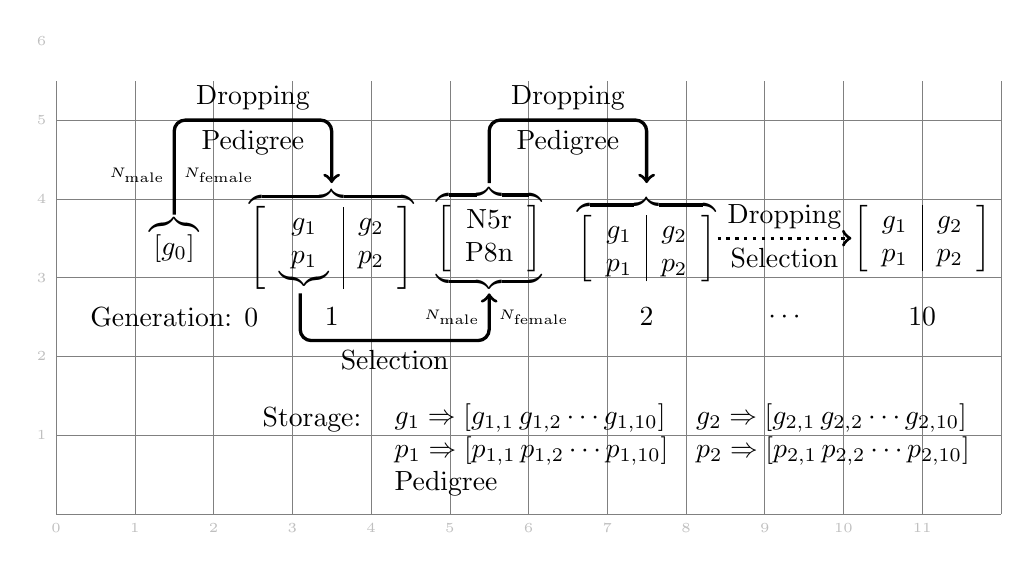
\begin{tikzpicture}
  %if to convert to jpg/png. but pdf is usually enougth.
  %convert -verbose -density 300 gs-data-structure.pdf -quality 100 -flatten -sharpen 0x1.0 t.jpg
  \draw[help lines] (0,0) grid (12,5.5);
  \foreach \x in {0, 1, ..., 11} \node[below, gray!50] at (\x,0){\tiny{\x}};
  \foreach \y in {1, 2, ..., 6} \node[left, gray!50] at (0,\y){\tiny{\y}};
  \node at (1.5, 3.5) {$\overbrace{\left[g_0\right]}$};
  \node at (1.5, 2.5) {Generation: 0};
  \node at (3.5, 3.5) {$\overbrace{\left[\begin{array}{c|c}g_1 & g_2 \\
        \underbrace{p_1} & p_2 \end{array}\right]}$};
  \node at (3.5, 2.5) {1};
  \node at (5.5, 3.5) {$\overbrace{\underbrace{\left[\begin{array}{c}
            \mathrm{N5r}\\\mathrm{P8n}\end{array}\right]}}$};
  \node at (7.5, 3.5) {$\overbrace{\left[\begin{array}{c|c}g_1 & g_2 \\
          p_1 & p_2 \end{array}\right]}$};
  \node at (7.5, 2.5) {2};
  \node at (11, 3.5) {$\left[\begin{array}{c|c}g_1 & g_2 \\
        p_1 & p_2 \end{array}\right]$};
  \node at (11, 2.5) {10};

  \draw[->, very thick, rounded corners] (1.5,3.8)--(1.5,5)--(3.5,5)--(3.5,4.2);
  \node[right] at (1.5, 4.3) {\tiny $N_{\mathrm{female}}$};
  \node[left] at (1.5, 4.3) {\tiny $N_{\mathrm{male}}$};
  \node[above] at (2.5, 5) {Dropping};
  \node[below] at (2.5, 5) {Pedigree};
  \draw[->, very thick, rounded corners] (3.1, 2.8)--(3.1, 2.2)--(5.5,2.2)--(5.5,2.8);
  \node[below] at (4.3, 2.2) {Selection};
  \node[right] at (5.5, 2.5) {\tiny $N_{\mathrm{female}}$};
  \node[left] at (5.5, 2.5) {\tiny $N_{\mathrm{male}}$};
  \draw[->, very thick, rounded corners] (5.5,4.2)--(5.5,5)--(7.5,5)--(7.5,4.2);
  \node[above] at (6.5, 5) {Dropping};
  \node[below] at (6.5, 5) {Pedigree};
  \draw[->, very thick, rounded corners, dotted] (8.4, 3.5)--(10.1, 3.5);
  \node[above] at (9.25, 3.5) {Dropping};
  \node[below] at (9.25, 3.5) {Selection};
  \node at (9.25, 2.5) {$\cdots$};
  \node[right] at (2.5, 1.2) {Storage:};
  \node[right] at (4, .8) {$\begin{array}{ll}
      g_1\Rightarrow[g_{1,1}\,g_{1,2}\cdots g_{1,10}] & g_2\Rightarrow[g_{2,1}\,g_{2,2}\cdots g_{2,10}]\\
      p_1\Rightarrow[p_{1,1}\,p_{1,2}\cdots p_{1,10}] & p_2\Rightarrow[p_{2,1}\,p_{2,2}\cdots p_{2,10}]\\
      \mathrm{Pedigree}
    \end{array}$};
\end{tikzpicture} 
\end{document}
